\documentclass{standalone}
\usepackage{times}
\usepackage{mathtools}

\usepackage{tikz}
\usetikzlibrary{positioning,fit,shapes,calc,decorations.pathreplacing}
\usetikzlibrary{backgrounds}
\usetikzlibrary{arrows.meta}
\usetikzlibrary{shapes,snakes}

\definecolor{processblue}{cmyk}{1,1,1,0}
\definecolor{accent}{rgb}{0.6,0.6,0.6}
\definecolor{accent2}{rgb}{0.9,0.9,0.9}
\definecolor{myblue}{rgb}{0.0,0.5,0.8}

\begin{document}
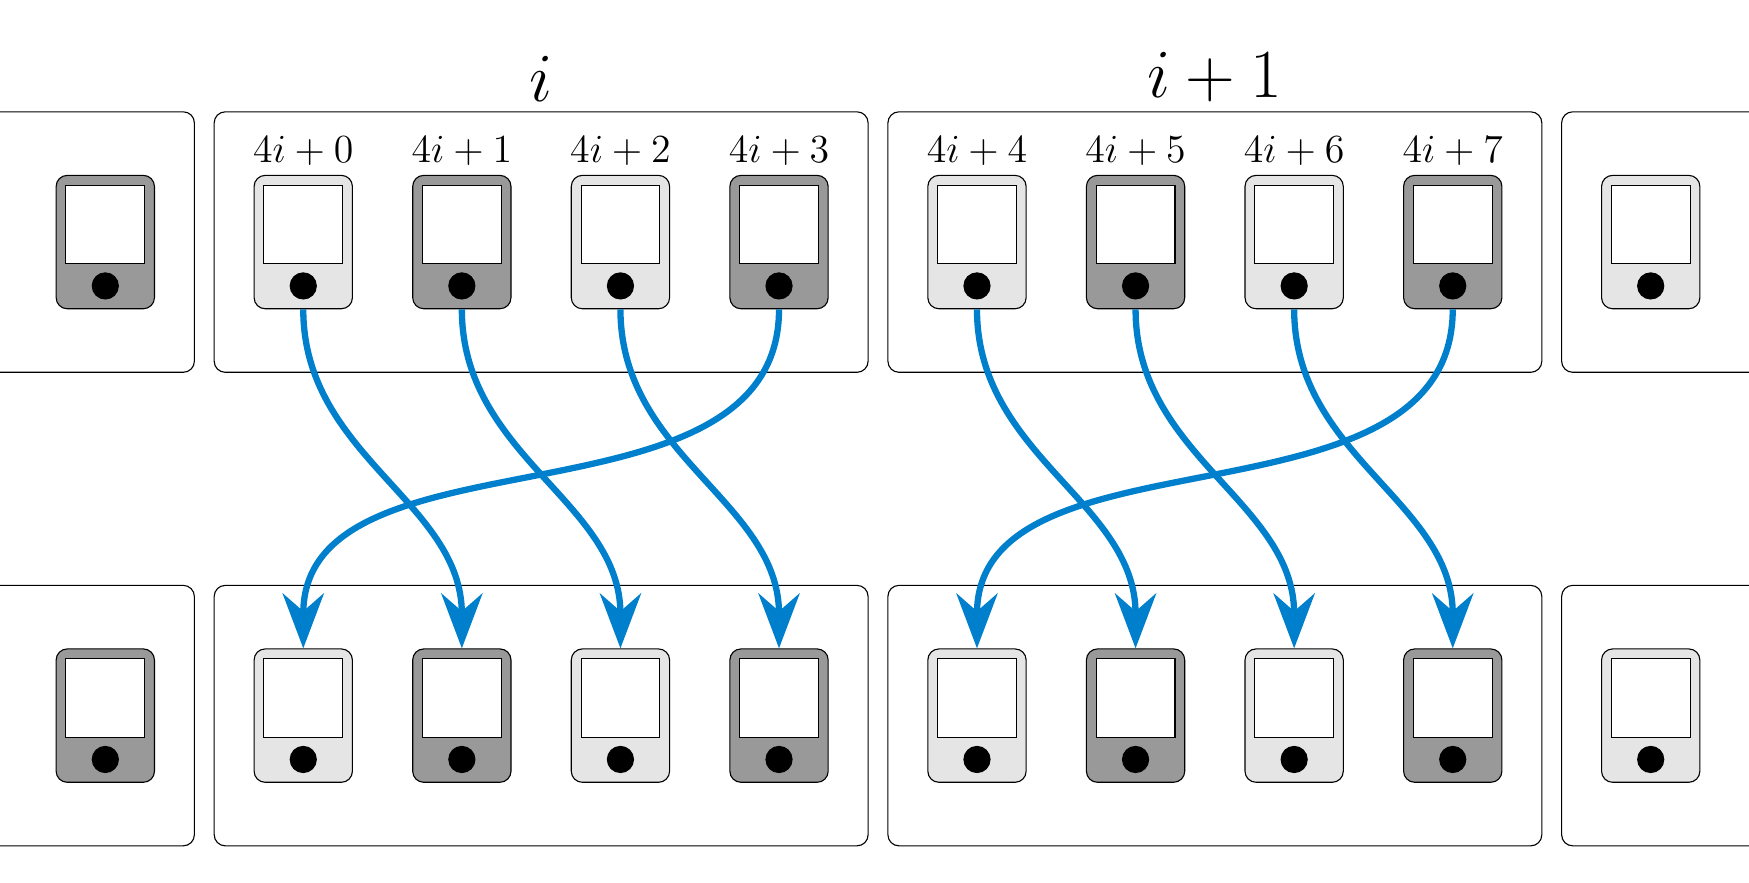
\begin{tikzpicture}[
  data/.style = {
    draw,
    rectangle,
    fill = white,
    minimum width = 1.0cm,
    minimum height = 1.0cm,
  },
  next/.style = {
    draw,
    circle,
    fill=black,
  },
  edge/.style = {
    draw,
    rectangle,
    rounded corners,
    minimum width = 0.5cm,
    minimum height = 0.5cm,
  },
  vedge/.style = {
    edge,
    top color = accent2,
    bottom color = accent2,
  },
  fedge/.style = {
    edge,
    top color = accent,
    bottom color = accent,
  },
  >={Stealth[scale=1.5]},
]

  \clip (-3.5,-8.0) rectangle (18,2.5);

  \node[data] (d0) {};
  \node[data] (d1) [right=of d0] {};
  \node[data] (d2) [right=of d1] {};
  \node[data] (d3) [right=of d2] {};

  \node[data] (d4) [right=1.5cm of d3] {};
  \node[data] (d5) [right=of d4] {};
  \node[data] (d6) [right=of d5] {};
  \node[data] (d7) [right=of d6] {};

  \node[data] (dl0) [left=1.5cm of d0] {};
  \node[data] (dl1) [left=of dl0] {};
  \node[data] (dr0) [right=1.5cm of d7] {};
  \node[data] (dr1) [right=of dr0] {};

  \node[next] (n0) [below=0.1cm of d0] {};
  \node[next] (n1) [below=0.1cm of d1] {};
  \node[next] (n2) [below=0.1cm of d2] {};
  \node[next] (n3) [below=0.1cm of d3] {};
  \node[next] (n4) [below=0.1cm of d4] {};
  \node[next] (n5) [below=0.1cm of d5] {};
  \node[next] (n6) [below=0.1cm of d6] {};
  \node[next] (n7) [below=0.1cm of d7] {};

  \node[next] (nl0) [below=0.1cm of dl0] {};
  \node[next] (nl1) [below=0.1cm of dl1] {};
  \node[next] (nr0) [below=0.1cm of dr0] {};
  \node[next] (nr1) [below=0.1cm of dr1] {};

  \begin{scope}[on background layer]
    \node[vedge,fit=(d0) (n0),label={\Large $4i+0$}] (e0) {};
    \node[fedge,fit=(d1) (n1),label={\Large $4i+1$}] (e1) {};
    \node[vedge,fit=(d2) (n2),label={\Large $4i+2$}] (e2) {};
    \node[fedge,fit=(d3) (n3),label={\Large $4i+3$}] (e3) {};
    \node[vedge,fit=(d4) (n4),label={\Large $4i+4$}] (e4) {};
    \node[fedge,fit=(d5) (n5),label={\Large $4i+5$}] (e5) {};
    \node[vedge,fit=(d6) (n6),label={\Large $4i+6$}] (e6) {};
    \node[fedge,fit=(d7) (n7),label={\Large $4i+7$}] (e7) {};

    \node[vedge,fit=(nl1) (dl1)] (el1) {};
    \node[fedge,fit=(nl0) (dl0)] (el0) {};
    \node[vedge,fit=(nr0) (dr0)] (er0) {};
    \node[fedge,fit=(nr1) (dr1)] (er1) {};
  \end{scope}

  \begin{scope}[on background layer]
    \node[draw,rectangle,fit=(e0) (e3),inner sep=0.5cm,inner ysep=0.8cm,rounded corners,label={\Huge $i$}] (q0) {};
    \node[draw,rectangle,fit=(e4) (e7),inner sep=0.5cm,inner ysep=0.8cm,rounded corners,label={\Huge $i+1$}] (q1) {};

    \node[draw,rectangle,fit=(el0) (el1),inner sep=0.5cm,inner ysep=0.8cm,rounded corners] (ql) {};
    \node[draw,rectangle,fit=(er0) (er1),inner sep=0.5cm,inner ysep=0.8cm,  rounded corners] (qr) {};
  \end{scope}


  % second part
  \node[data] (td0) [below=5cm of d0] {};
  \node[data] (td1) [right=of td0] {};
  \node[data] (td2) [right=of td1] {};
  \node[data] (td3) [right=of td2] {};

  \node[data] (td4) [right=1.5cm of td3] {};
  \node[data] (td5) [right=of td4] {};
  \node[data] (td6) [right=of td5] {};
  \node[data] (td7) [right=of td6] {};

  \node[data] (tdl0) [left=1.5cm of td0] {};
  \node[data] (tdl1) [left=of tdl0] {};
  \node[data] (tdr0) [right=1.5cm of td7] {};
  \node[data] (tdr1) [right=of tdr0] {};

  \node[next] (tn0) [below=0.1cm of td0] {};
  \node[next] (tn1) [below=0.1cm of td1] {};
  \node[next] (tn2) [below=0.1cm of td2] {};
  \node[next] (tn3) [below=0.1cm of td3] {};
  \node[next] (tn4) [below=0.1cm of td4] {};
  \node[next] (tn5) [below=0.1cm of td5] {};
  \node[next] (tn6) [below=0.1cm of td6] {};
  \node[next] (tn7) [below=0.1cm of td7] {};

  \node[next] (tnl0) [below=0.1cm of tdl0] {};
  \node[next] (tnl1) [below=0.1cm of tdl1] {};
  \node[next] (tnr0) [below=0.1cm of tdr0] {};
  \node[next] (tnr1) [below=0.1cm of tdr1] {};

  \begin{scope}[on background layer]
    \node[vedge,fit=(td0) (tn0)] (te0) {};
    \node[fedge,fit=(td1) (tn1)] (te1) {};
    \node[vedge,fit=(td2) (tn2)] (te2) {};
    \node[fedge,fit=(td3) (tn3)] (te3) {};
    \node[vedge,fit=(td4) (tn4)] (te4) {};
    \node[fedge,fit=(td5) (tn5)] (te5) {};
    \node[vedge,fit=(td6) (tn6)] (te6) {};
    \node[fedge,fit=(td7) (tn7)] (te7) {};

    \node[vedge,fit=(tnl1) (tdl1)] (tel1) {};
    \node[fedge,fit=(tnl0) (tdl0)] (tel0) {};
    \node[vedge,fit=(tnr0) (tdr0)] (ter0) {};
    \node[fedge,fit=(tnr1) (tdr1)] (ter1) {};
  \end{scope}

  \begin{scope}[on background layer]
    \node[draw,rectangle,fit=(te0) (te3),inner sep=0.5cm,inner ysep=0.8cm,rounded corners] (tq0) {};
    \node[draw,rectangle,fit=(te4) (te7),inner sep=0.5cm,inner ysep=0.8cm,rounded corners] (tq1) {};

    \node[draw,rectangle,fit=(tel0) (tel1),inner sep=0.5cm,inner ysep=0.8cm,rounded corners] (tql) {};
    \node[draw,rectangle,fit=(ter0) (ter1),inner sep=0.5cm,inner ysep=0.8cm,  rounded corners] (tqr) {};
  \end{scope}


  \path[->,myblue,line width=0.8mm] (e0) edge[out=-90,in=90] node {} (te1);
  \path[->,myblue,line width=0.8mm] (e1) edge[out=-90,in=90] node {} (te2);
  \path[->,myblue,line width=0.8mm] (e2) edge[out=-90,in=90] node {} (te3);
  \path[->,myblue,line width=0.8mm] (e3) edge[out=-90,in=90] node {} (te0);

  \path[->,myblue,line width=0.8mm] (e4) edge[out=-90,in=90] node {} (te5);
  \path[->,myblue,line width=0.8mm] (e5) edge[out=-90,in=90] node {} (te6);
  \path[->,myblue,line width=0.8mm] (e6) edge[out=-90,in=90] node {} (te7);
  \path[->,myblue,line width=0.8mm] (e7) edge[out=-90,in=90] node {} (te4);

\end{tikzpicture}
\end{document}
